\section{Numerical Results}
\label{sec:numRes}
We now have some MFT predictions about the SPM, and a few ideas about when those predictions might be invalid. Thus, we test them out numerically.
We chose to calculate using the \texttt{KMCLib}\cite{leetmaa2014kmclib} package, which implements the Kinetic Monte Carlo algorithm
(essentially the same as the Gillespie algorithm\cite{Gillespie1977})
on lattice systems. The codes used are kept here~\cite{jHellGitRepo}.
%\texttt{KMCLib} has the advantage that it is python-wrapped \texttt{C++}, and thus quite easy to use whilst at the same time being quite computationally efficient; thus it was fairly easy for us to carry out large numbers
%of differently-parametrised serial \texttt{KMCLib} jobs on the \texttt{Eddie3} computing cluster here at Edinburgh. 
As we have MFT predictions about flow in a block, we can simulate that situation using KMC. In the bulk, the transition rates are simply those described in Figure~\ref{fig:rates}. At the boundaries, referred to as the ``top''  and ``bottom''
of the block, there are 2 layers of lattice sites what switch between being full and empty with rates such that the time-averaged occupation can be specified to match the desired boundary conditions; there are then chances for particles to spawn
and despawn with rates depending upon the occupation of these boundary layers. In the end, the intention is that these boundaries should reproduce the effect of having particle reservoirs attached to the ends, which is something we check
in the output by inspecting the time-averaged occupations of sites near the boundary. We have used this setup to explore three scenarios, discussed in the following sections. In each of these we refer to a boundary condition configuration
by $(\rho_0, \rho_L)$, with $\rho_0$ and $\rho_L$ being the bottom and top boundary densities respectively.
When we measure flow rate in such a situation, we perform a specified number of Gillespie steps and count the number of particles entering at the top $e_L$, leaving at the top $l_L$, entering at the bottom $e_0$, leaving at the bottom $l_0$,
as well as the Gillespie time interval $T$ that elapses during those steps; we then have an estimate of the overall flow rate $J$ via
\begin{equation}
 J = \frac{e_0-e_L+l_L-l_0}{2T}.
\end{equation}
We can also calculate the time-averaged total number of particles in the system; this is done by updating a histogram of particle numbers
as the simulation progresses. In each of our calculations, we make the initial configuration by randomly filling the system with particles and vacancies in such a way that the initial density should be $\frac{1}{2}(\rho_0 + \rho_L)$, and then
run the system for a sufficient number of equilibration steps to destroy any initial transients.

The MFT suggests that a  transition, from a steady flow regime to a critically slow flow regime, might occur as the stickiness varies.
We test this by holding the boundary densities constant
whilst changing $\lambda$, and measuring the particle density as well as the mean, variance and skewness of the flow rate. If such a transition does indeed occur, we should expect to see a divergence in one of these moments.
We have done this with 4 sets of boundary conditions as shown in Figure~\ref{fig:lambdaScans}. 
\begin{figure*}[h!]
\vspace{1em}
\caption{\label{fig:lambdaScans} Moments of flow rates and average overall densities observed when varying $\lambda$ with fixed boundary densities $(\rho_0, \rho_L)$: Blue refers to $(\frac{2}{3}, \frac{2}{3})$, yellow to $(\frac{3}{4}, \frac{7}{12})$
(both with average density $\frac{2}{3}$); green to $(\frac{3}{4}, \frac{1}{4})$, red to $(\frac{99}{100}, \frac{1}{100})$ (with average density $\frac{1}{2}$). In the case of the mean flow we have an MFT prediction, indicated by the solid line.
In each case we used systems of length $64$ (length $32$ gives similar results),
running them for $400000$ Gillispie steps for equilibration followed by $10000$ measurement runs of $1000$ steps interspersed with relaxation runs of $16000$
steps. This way we could gather statistics about flow rates and densities in a well-equilibrated system. Specifically, we generate a pool of $10000$ samples of flow rate and density,
from which we can calculate estimates of the descriptive statistics of both quantities.}
\begin{center}
 \begin{tabular}{c|c}
    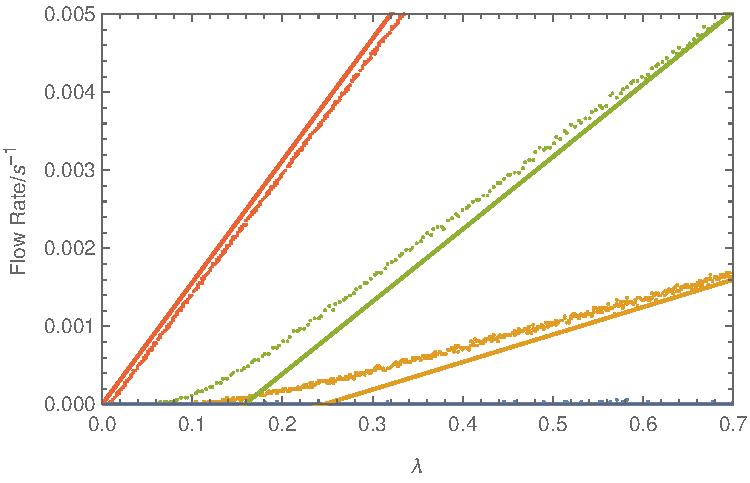
\includegraphics[width=0.5\linewidth]{../tex-src/images/lambdaScan/flowMean} & 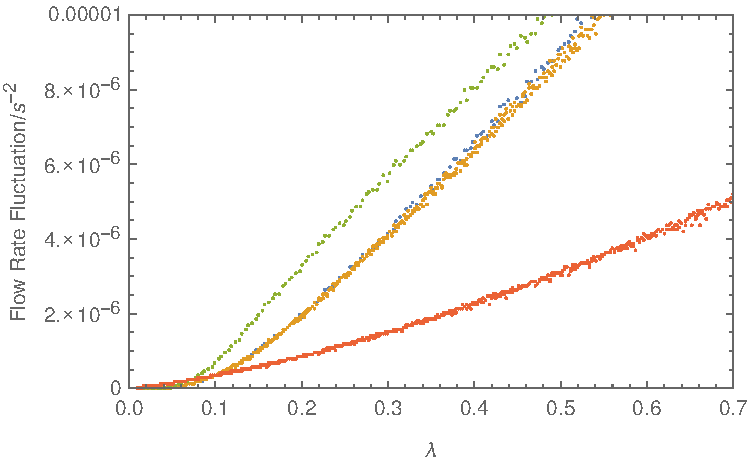
\includegraphics[width=0.5\linewidth]{../tex-src/images/lambdaScan/flowVar} \\
    \hline
    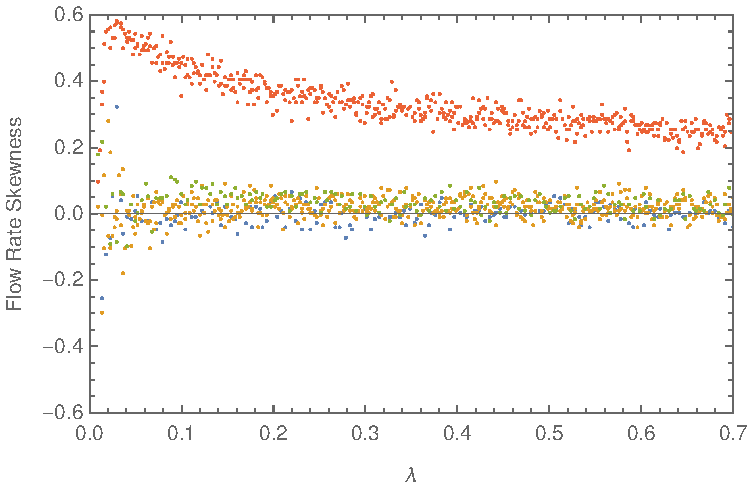
\includegraphics[width=0.5\linewidth]{../tex-src/images/lambdaScan/flowSkew} & 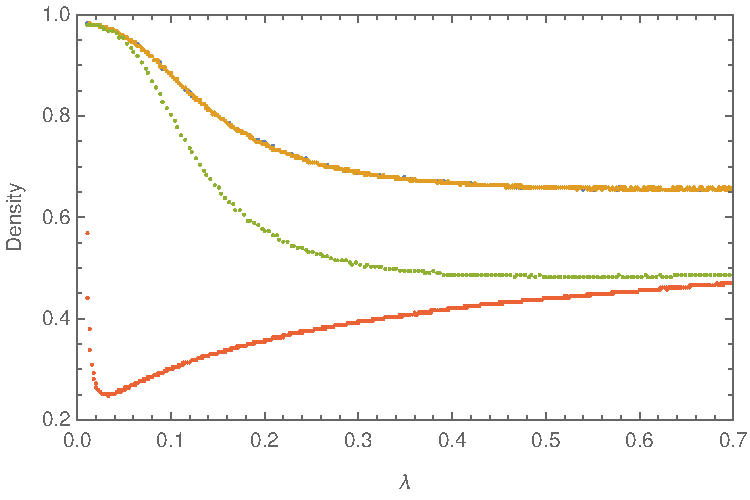
\includegraphics[width=0.5\linewidth]{../tex-src/images/lambdaScan/lambdaDens} \\
    \end{tabular}
\end{center}
    \vspace{-0em}
\end{figure*}

Firstly, we should note that we only have an MFT prediction for the flow rate as a function of $\lambda$ as  $\rho(x)$ stops being unique when $\lambda$ drops below $\frac{1}{4}$,
and so the MFT lacks predictive power. For low-stickiness, when $\lambda>\frac{1}{4}$, the MFT is in good agreement with the simulations.
However, one of the key predictions of the MFT, that a sharp transition to a no-flow regime occurs when $\lambda$ becomes small enough (at least for 3 of the 4 sets of
boundary conditions we investigated here), does not seem to be realised in our simulations. Indeed what seems to be happening is that the sharp transition has been smoothed out, as we
do not see any peaks or jumps in the flow rate variance or skewness, which we would expect to see if there was a transition. We suspect that this discrepancy is due to nontrivial correlations emerging between the particles, which the MFT
does not take account of for obvious reasons. Alternatively, it could be that the continuum assumption is failing due to the (finite-sized) system filling with particles and blocking.
As for the observed average density, for larger $\lambda$ the density approaches the average of the boundary densities,
and for small $\lambda$ the density approaches $1$ (which makes sense as the particles are very strongly attracted to each other, and so the system has a tendency to fill up); the exception to this it the case with extreme full/empty boundary
conditions, although in this case one might argue that the particles are ``sucked out'' of the system so rapidly at the empty end that the system never really has a chance to fill up. It is also worth noticing that this extreme case is the only
one in which the flow rate skewness does anything interesting; it is mostly positive, especially at low-$\lambda$, implying that most of the time the system is fairly static, but occasionally short-lived strong flows occur which end up causing
most of the bulk flow.

Another situation we can investigate has boundaries $(\rho_B, \rho_T) = (\rho_M + \frac{1}{2} \delta\rho, \rho_M - \frac{1}{2} \delta\rho)$ for some given $\rho_M$, where $\delta\rho$ and $\lambda$ are varied. As before, I calculated flow rate
moments and average densities, and the results are displayed in Figure~\ref{fig:constDens}. 
\begin{figure*}[h!]
\vspace{1em}
\caption{\label{fig:constDens} Flow rate mean, flow variance and average overall densities observed when varying the difference $\delta\rho$ between the boundary concentrations
$(\rho_B, \rho_T) = (\rho_M + \frac{1}{2} \delta\rho, \rho_M - \frac{1}{2} \delta\rho)$ and $\lambda$. I chose $\rho_M=\frac{1}{2}$, as this gives us the biggest range of $\delta\rho$ to investigate.
These calculations were performed with the same run parameters (system length etc)
as above. The top left panel is the MFT prediction
for the flow rate, whilst top right shows the observed mean flow rate. The measured flow skewness and kurtosis are not displayed here as both signals were small and noisy, and didn't show anything particularly significant.}
\begin{center}
 \begin{tabular}{c|c}
    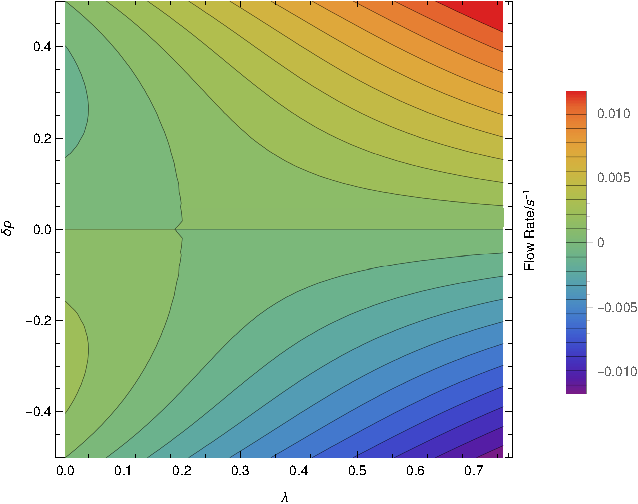
\includegraphics[width=0.5\linewidth]{../tex-src/images/constDens/constAnalFlow-crop} & 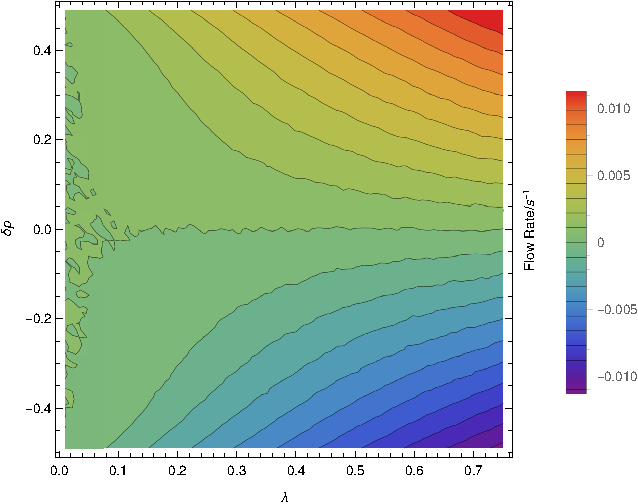
\includegraphics[width=0.5\linewidth]{../tex-src/images/constDens/meanFlowContour-crop} \\
    \hline
    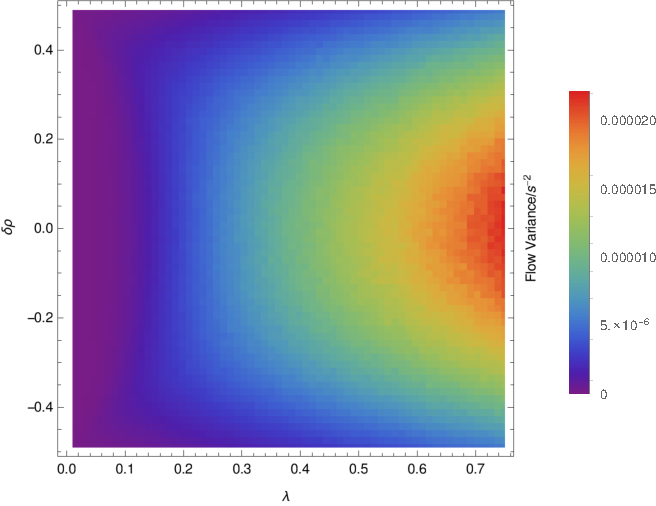
\includegraphics[width=0.5\linewidth]{../tex-src/images/constDens/varFlow-crop} & 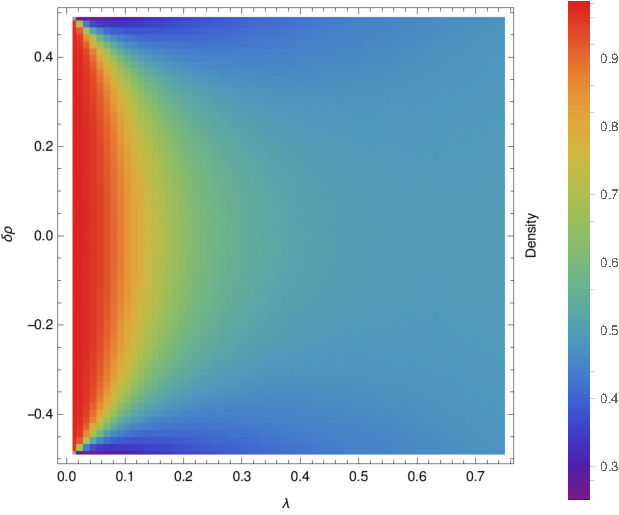
\includegraphics[width=0.5\linewidth]{../tex-src/images/constDens/meanDens-crop} \\
    \end{tabular}
\end{center}
    \vspace{-0em}
\end{figure*}
The MFT prediction for the mean flow is generally in good agreement with the numerics, except in the very sticky regime in which flow is very small.
The simulations show no evidence of negative diffusion; rather the flow becomes critically slow for very sticky particles.
The higher moments of the flow (e.g. variance, Figure~\ref{fig:constDens} bottom left) do not show peaks, indicating that hard transitions aren’t occurring.
Finally (bottom right), the density is very close to the average of the boundary densities until λ drops below 1/4, at which point the stickiness causes the system to fill.


\subsection{Diffusion Coefficient Measurement}
Let us again specify the boundary densities to be $(\rho_0, \rho_L) = (\rho_M + \frac{1}{2} \delta\rho, \rho_M - \frac{1}{2} \delta\rho)$ for some given $\rho_M$. This time we keep $\delta\rho$ relatively small, so that $J$ varies approximately
linearly with $\delta\rho$; thus if we calculate $J$ for a series of small $\delta \rho$, we can perform linear regression to find $D=\partDeriv{J}{\delta\rho}\big|_{\delta\rho=0}$, the effective diffusion coefficient.
Computing this for different $(\rho_M, \lambda)$ combinations yields results that can be compared with Equation~\ref{eq:MFTflow}.
\begin{figure*}[h!]
\vspace{1em}
\caption{\label{fig:diffCoef} The contour plot on the left shows the MFT prediction of the diffusion coefficient $D=\partDeriv{J}{\delta\rho}\big|_{\delta\rho=0}$ as a function of local density $\rho_M$ and $\lambda$;
we are only plotting where $0 \le D \le 1.2$, other regions are shown in white, including the region in which $D<0$, which would cause instabilities and so prevent a flow from actually occurring.
On the right is our numerical calculation of $D(\rho_M, \lambda)$,
with exactly the same plotting ranges. The dots indicate which points in $(\rho_M, \lambda)$ we calculated $D$ around, to give an impression of how the interpolation in the contour plot was done.}
\begin{center}
 \begin{tabular}{c@{\hspace{1em}}c}
    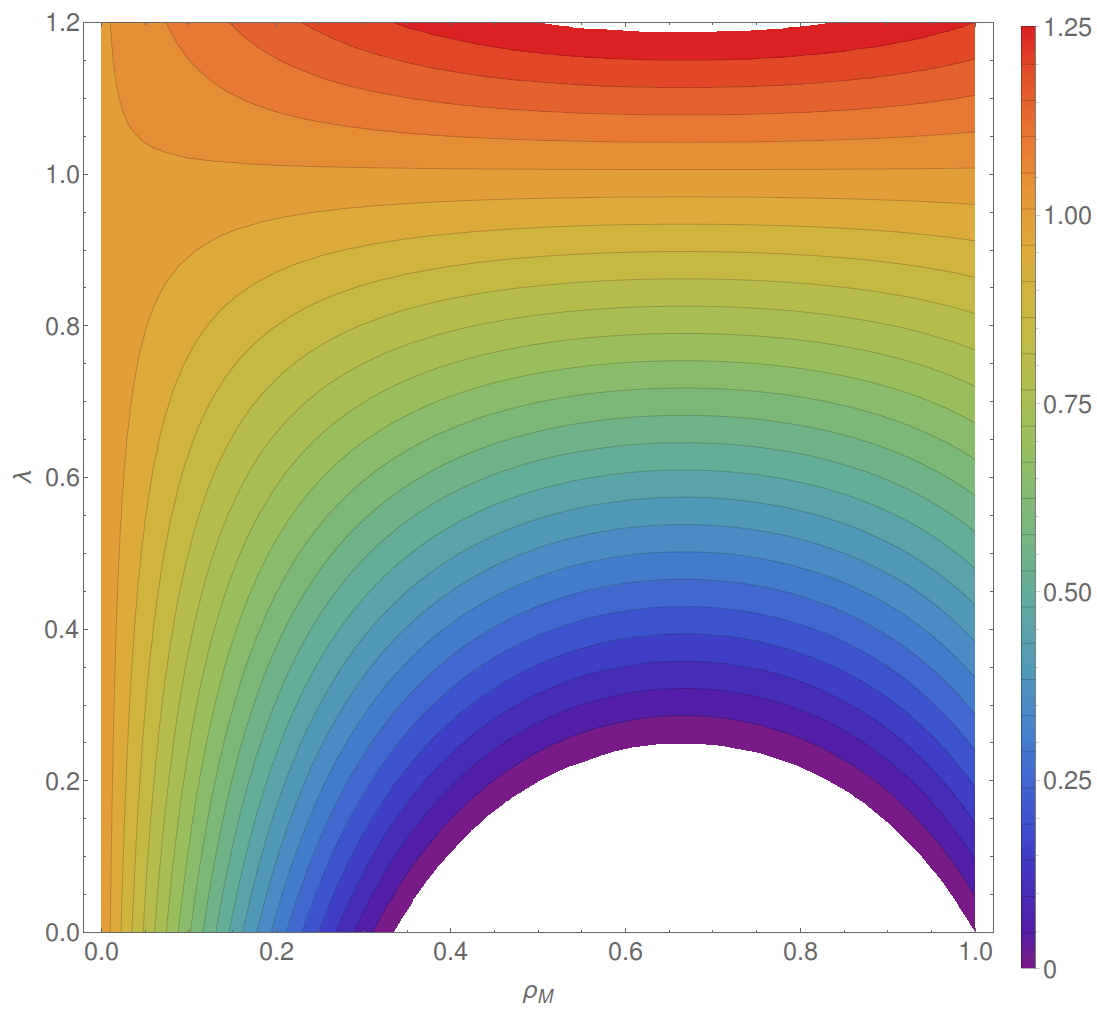
\includegraphics[width=0.5\linewidth]{../tex-src/images/analFlow.png} & 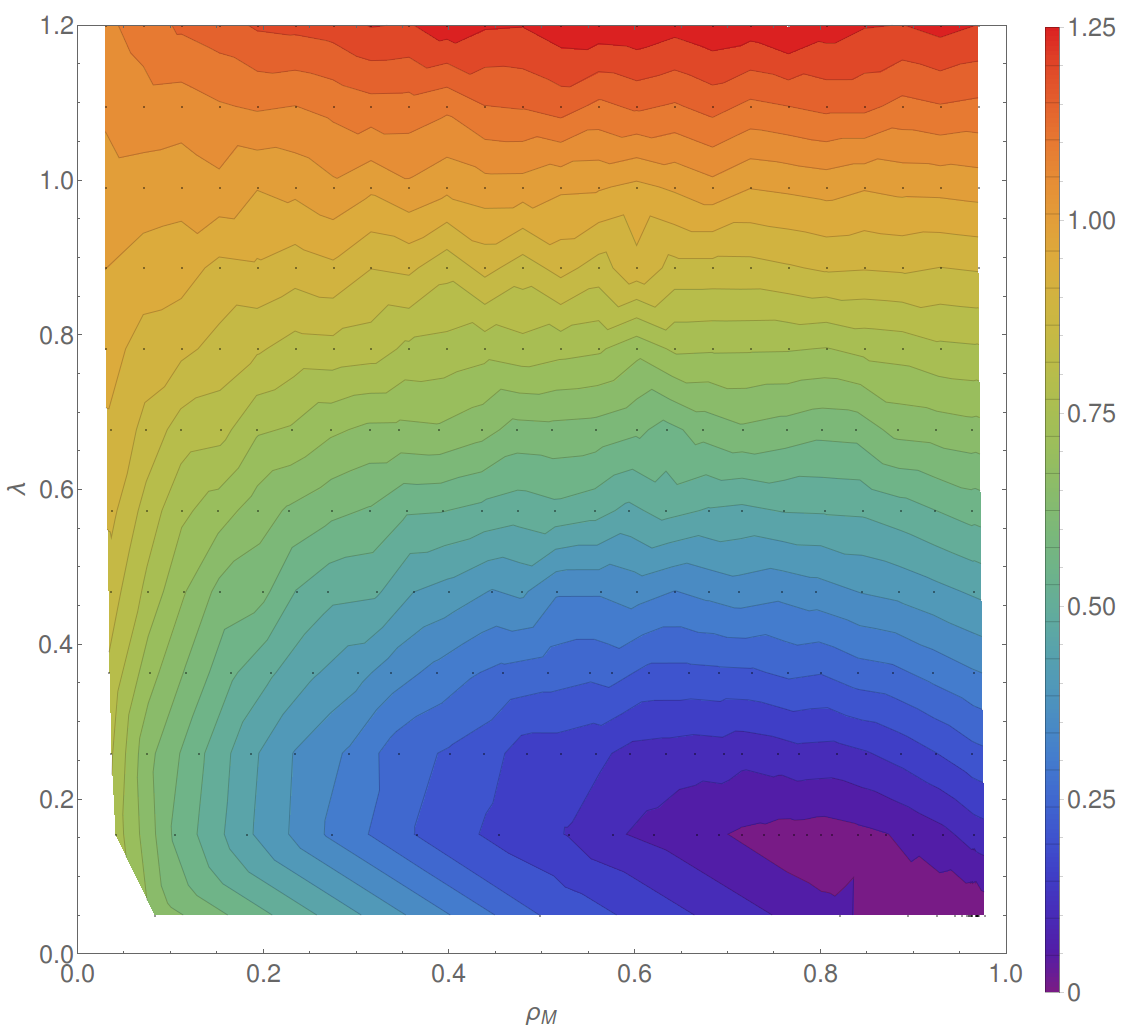
\includegraphics[width=0.5\linewidth]{../tex-src/images/dataFlow.png} \\
    \end{tabular}
\end{center}
    \vspace{-0em}
\end{figure*}
In this setup we ran the simulation for
$1.6\times10^8$ equilibration steps, followed by $10$ sets of alternating measurement and relaxation runs, of lengths $8\times10^7$ and $1.6\times10^7$ steps respectively. We repeated the calculation with a system of half the size, and again
found little difference between the two datasets, which gives us confidence that finite-size effects are small.
We can of course obtain estimates of the confidence interval for our linear regression coefficient, and thus generate a standard error for $D$; likewise we can obtain goodness of fit estimates for the
regression. They are not included here for brevity, but they are in the additional materials.
%REMEMBER TO ACTUALLY PUT IT THERE!!!

Putting the MFT prediction and the actual numerical results together as we have done in Figure~\ref{fig:diffCoef}, we can compare and contrast. We see that MFT and simulation agree well for low stickiness, and both show the strange symmetry
about $ρ_M = \frac{2}{3}$. For high stickiness, where the MFT prediction gives negative diffusion constant, the simulation generates a much increased density in the system.  This takes $ρ_M$ outside the negative-$D$ regime of the MFT,
and into slow, but positive $D$. 
%Query
The incorrectness of the MFT prediction suggests that some kind of nontrivial
correlations have built up in this region, which makes sense as the coupling between particles has become stronger, whilst the density is middling, allowing that coupling to mean something. It is also worth noting that the discrepancy between
intended density and actual density starts to become non-negligible here, which we can infer from how the originally rectangular grid of grey dots
(indicating $(\rho_M, \lambda)$ points where we obtained the data) has been deformed, to the extent that there is a big cluster of them in the observed minimum of the diffusion coefficient. Some of these anomalous densities are greater
than the density of the denser reservoir to which the system is coupled; thus, the reservoirs involved are in some sense ``unphysical'' as the data suggests that they would immediately attempt to switch to a higher density, which given a
constant volume constraint would imply a phase separation occurs; thus the numerical results aren't fitting so well into the paradigm we were using to analyse them (flow between reservoirs with slightly different densities),
so it's little wonder the MFT is having trouble keeping up. Of course, we do not see the negative diffusion coefficient that naive application of MFT would suggest, because it would cause instability; instead, the diffusion coefficient just
becomes very small, as the system becomes unresponsive to concentration gradients.

\subsection{Flow Structure}
\label{sec:flowStruc}
Figure~\ref{fig:flowPatterns} shows the short-time-averaged local density as a function of space and time for a range of densities and stickiness.
\iffalse
\begin{figure*}[h!]
\caption{\label{fig:flowPatterns} The spacetime flow patterns, for the $(\lambda, \rho_M)$ combinations indicated in the row and column headers. In each plot time runs along the $x$-axis, space along the $y$-axis. White represents full occupation, black empty, and grey shades partial
occupation. The degree of occupation was calculated by taking the \texttt{KMCLib} record of a particular site's occupation (i.e. the Gillespie times at
which the site changed occupation), assigning $0$ and $1$ to particles and vacancies respectively, linearly interpolating this and then integrating over times longer than a single Gillespie step but much shorter than the total time in question.
In each case the total time elapsed is that taken by $10^6$ Gillespie steps, and each short-time-average has been done over the total time divided by $508$ (to produce square diagrams, as there are $508$ active sites
per simulation). I chose to rescale time this way because if we used equal times it would appear that nothing happens in the low-$\lambda$ simulations, which isn't true!}
\begin{tabular}{c p{0.175\linewidth}}
\hspace{-2em}\begin{tabular}{c|c@{\hspace{0.25em}}c@{\hspace{0.25em}}c@{\hspace{0.25em}}c  }
  &  $\lambda=0.05$ & $\lambda=0.25$ & $\lambda=0.50$ & $\lambda=0.70$ \\ 
  \hline
   \begin{tabular}{c} \vspace{-12em} \\ \hspace{-1em}$\rho_M=0.05$\hspace{0em} \\  \\ \end{tabular} & 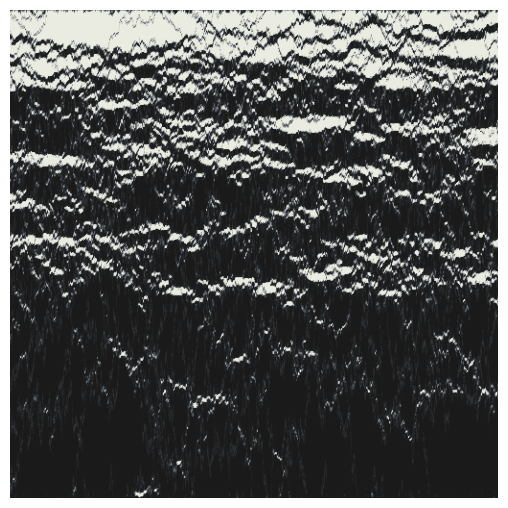
\includegraphics[width=0.24\linewidth]{../tex-src/images/flowImps/flowl0r0.png} & 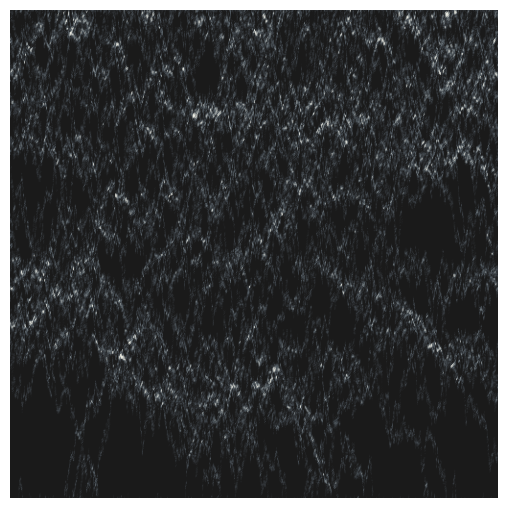
\includegraphics[width=0.24\linewidth]{../tex-src/images/flowImps/flowl1r0.png}  & 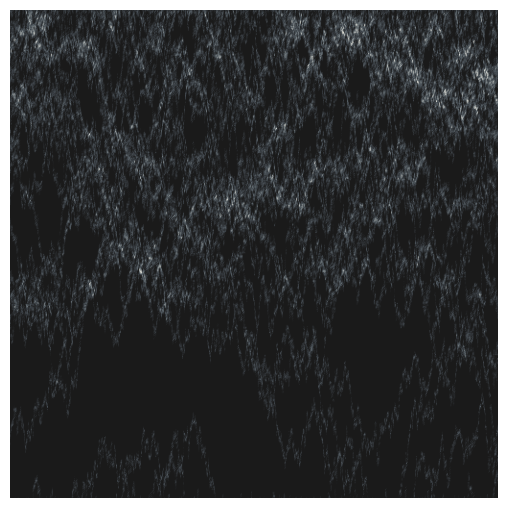
\includegraphics[width=0.24\linewidth]{../tex-src/images/flowImps/flowl2r0.png} & 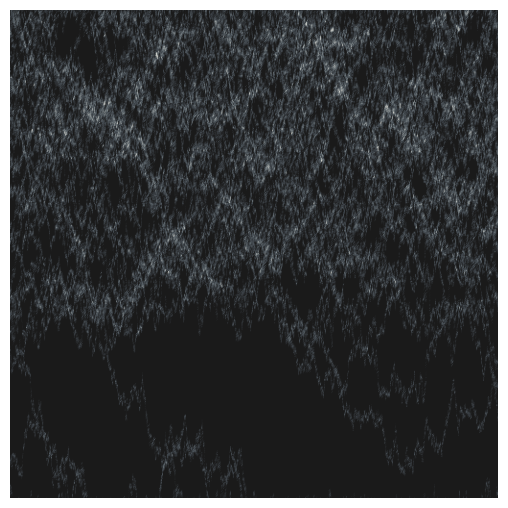
\includegraphics[width=0.24\linewidth]{../tex-src/images/flowImps/flowl3r0.png} \\
   \begin{tabular}{c} \vspace{-12em} \\ \hspace{-1em}$\rho_M=0.35$\hspace{0em} \\  \\ \end{tabular} & 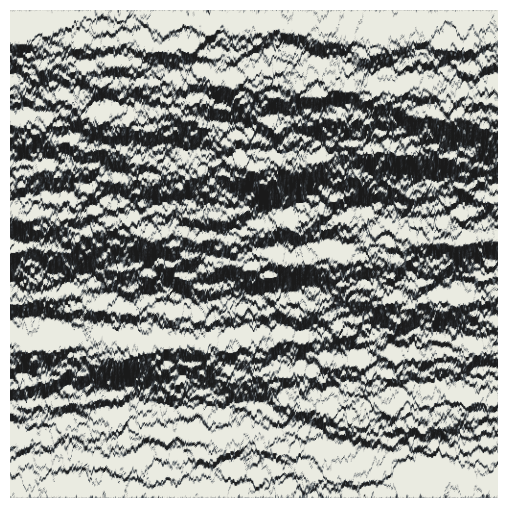
\includegraphics[width=0.24\linewidth]{../tex-src/images/flowImps/flowl0r1.png} & 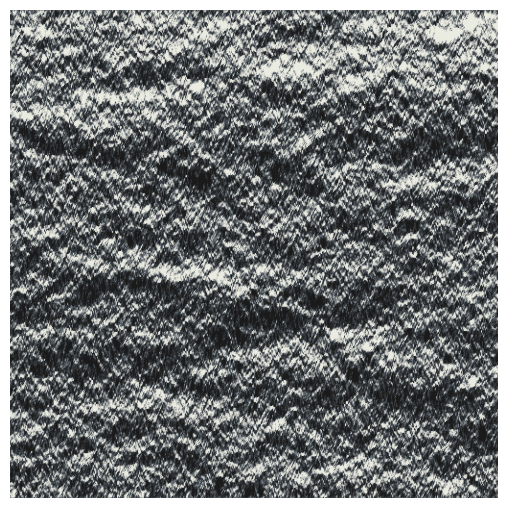
\includegraphics[width=0.24\linewidth]{../tex-src/images/flowImps/flowl1r1.png}  & 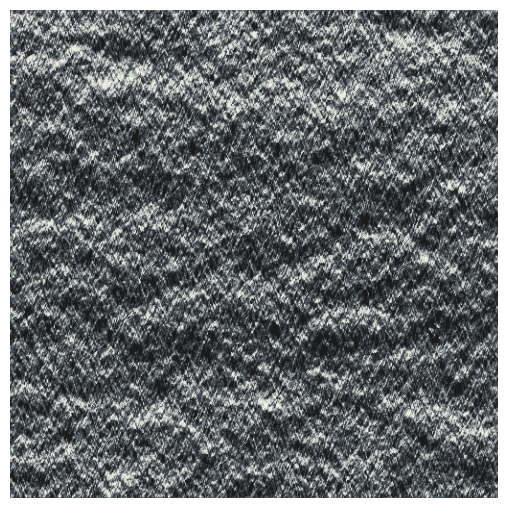
\includegraphics[width=0.24\linewidth]{../tex-src/images/flowImps/flowl2r1.png} & 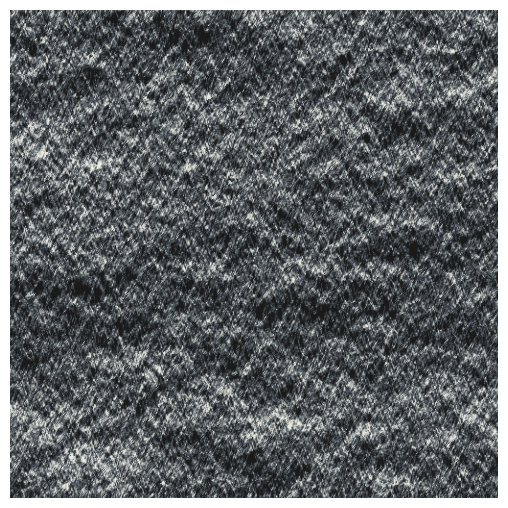
\includegraphics[width=0.24\linewidth]{../tex-src/images/flowImps/flowl3r1.png} \\
   \begin{tabular}{c} \vspace{-12em} \\ \hspace{-1em}$\rho_M=0.65$\hspace{0em} \\  \\ \end{tabular} & 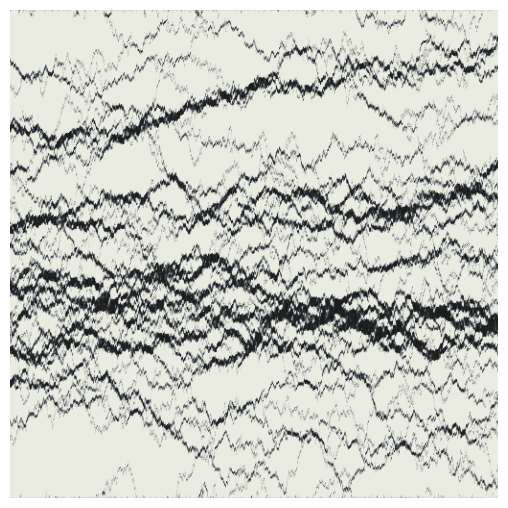
\includegraphics[width=0.24\linewidth]{../tex-src/images/flowImps/flowl0r2.png} & 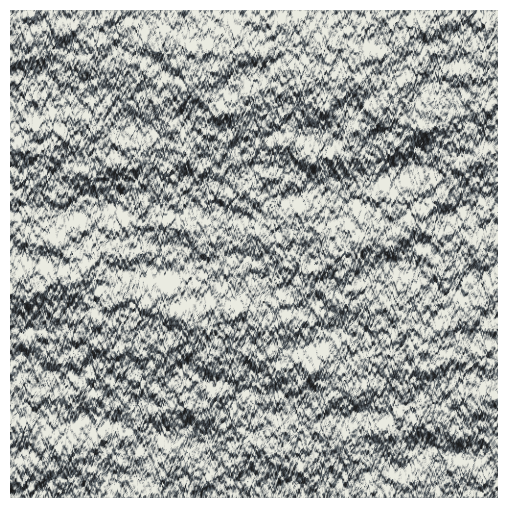
\includegraphics[width=0.24\linewidth]{../tex-src/images/flowImps/flowl1r2.png}  & 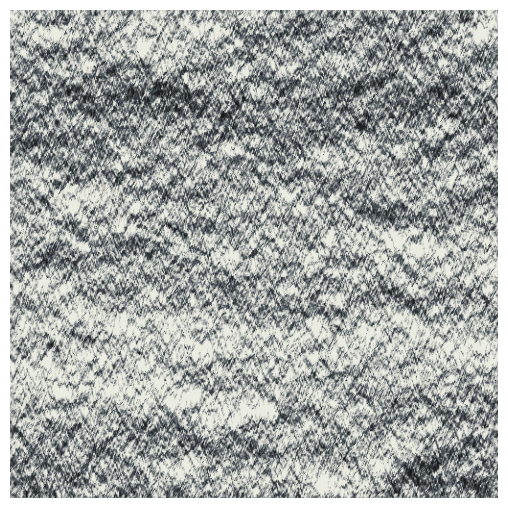
\includegraphics[width=0.24\linewidth]{../tex-src/images/flowImps/flowl2r2.png} & 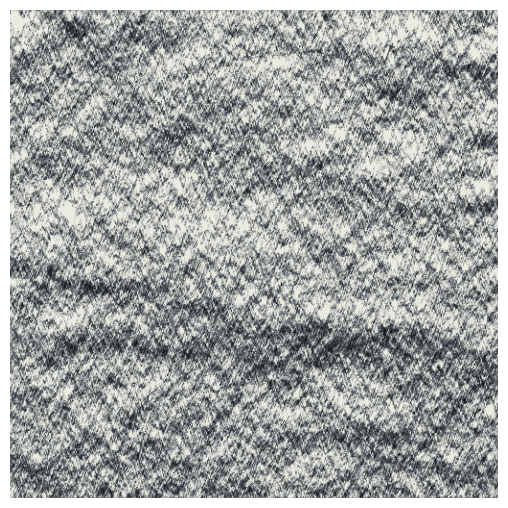
\includegraphics[width=0.24\linewidth]{../tex-src/images/flowImps/flowl3r2.png} \\
   \begin{tabular}{c} \vspace{-12em} \\ \hspace{-1em}$\rho_M=0.95$\hspace{0em} \\  \\ \end{tabular} & 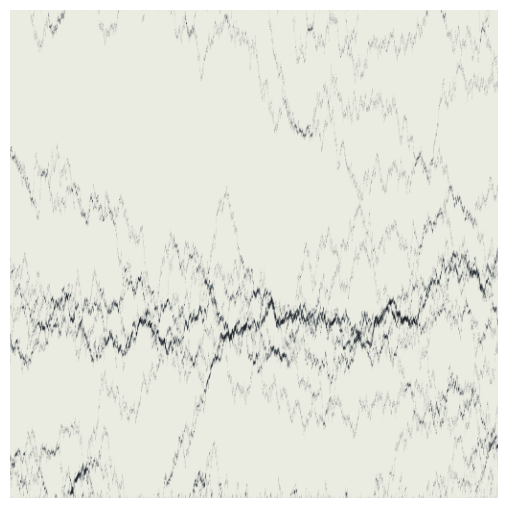
\includegraphics[width=0.24\linewidth]{../tex-src/images/flowImps/flowl0r3.png} & 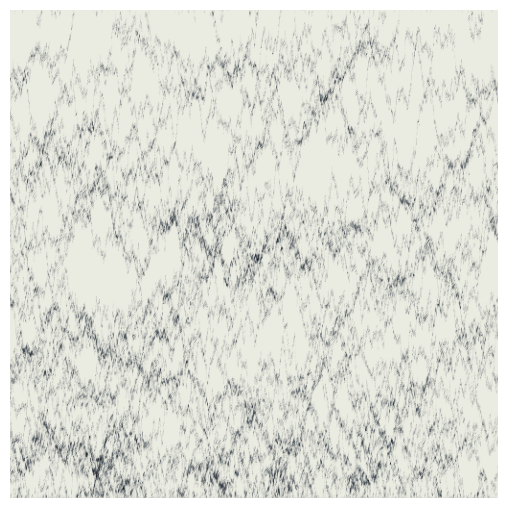
\includegraphics[width=0.24\linewidth]{../tex-src/images/flowImps/flowl1r3.png}  & 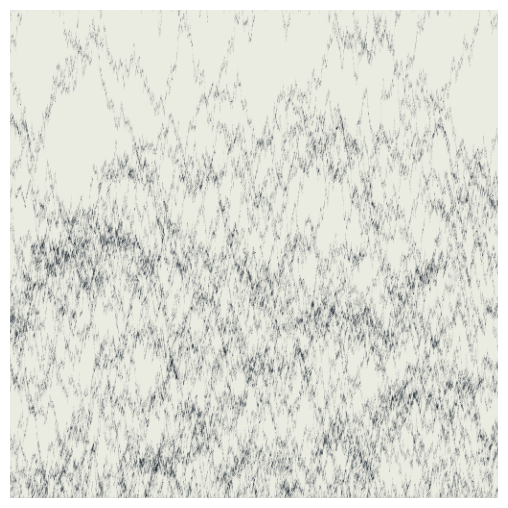
\includegraphics[width=0.24\linewidth]{../tex-src/images/flowImps/flowl2r3.png} & 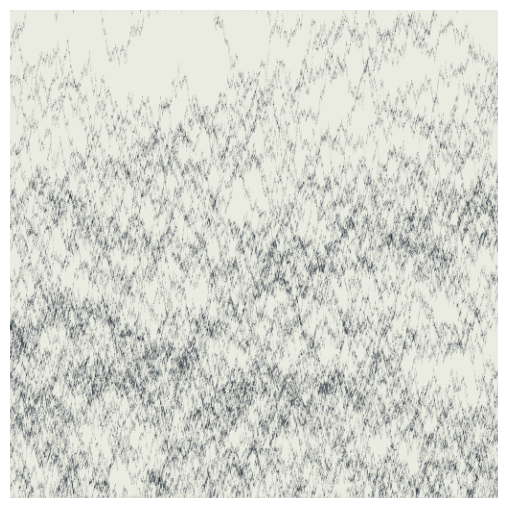
\includegraphics[width=0.24\linewidth]{../tex-src/images/flowImps/flowl3r3.png} \\
   \end{tabular}
\hspace{-1em}
&
\end{tabular}
\end{figure*}
\fi
\begin{figure*}[h!]
\caption{\label{fig:flowPatterns} The spacetime flow patterns, for the $(\lambda, \rho_M)$ combinations indicated in the row and column headers. In each plot time runs along the $x$-axis, space along the $y$-axis. White represents full occupation, black empty, and grey shades partial
occupation. The degree of occupation was calculated by taking the \texttt{KMCLib} record of a particular site's occupation (i.e. the Gillespie times at
which the site changed occupation), assigning $0$ and $1$ to particles and vacancies respectively, linearly interpolating this and then integrating over times longer than a single Gillespie step but much shorter than the total time in question.
In each case the total time elapsed is that taken by $10^6$ Gillespie steps, and each short-time-average has been done over the total time divided by $508$ (to produce square diagrams, as there are $508$ active sites
per simulation). Time has been rescaled this way in order to allow fair comparison of radically different $\lambda$-values.}
\begin{tabular}{c p{0.175\linewidth}}
\hspace{-2em}\begin{tabular}{c|c@{\hspace{0.25em}}c@{\hspace{0.25em}}c}
  &  $\lambda=0.05$ & $\lambda=0.38$ & $\lambda=1.00$ \\ 
  \hline
   \begin{tabular}{c} \vspace{-12em} \\ \hspace{-1em}$\rho_M=0.05$\hspace{0em} \\  \\ \end{tabular} & 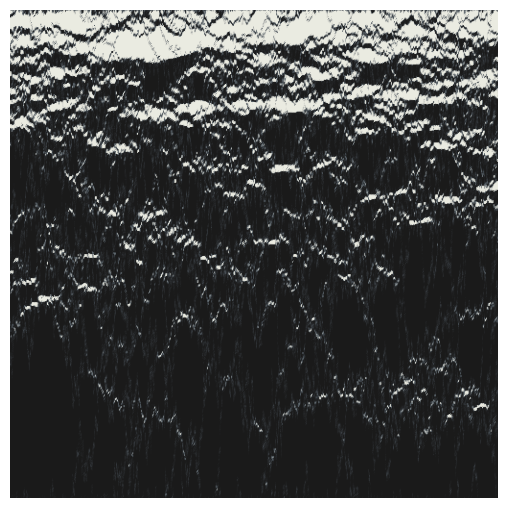
\includegraphics[width=0.32\linewidth]{../tex-src/images/flowImps2/flowl0r0.png} & 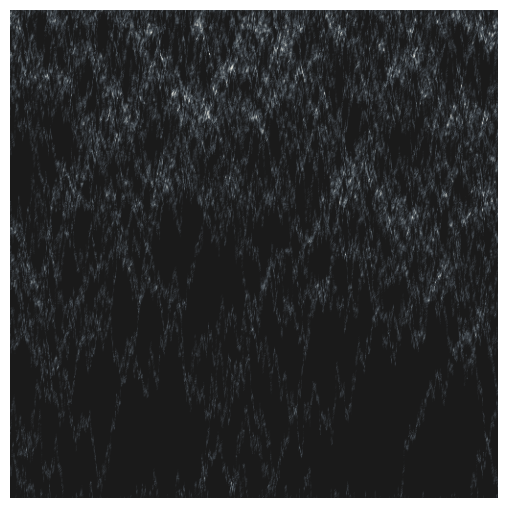
\includegraphics[width=0.32\linewidth]{../tex-src/images/flowImps2/flowl2r0.png}  & 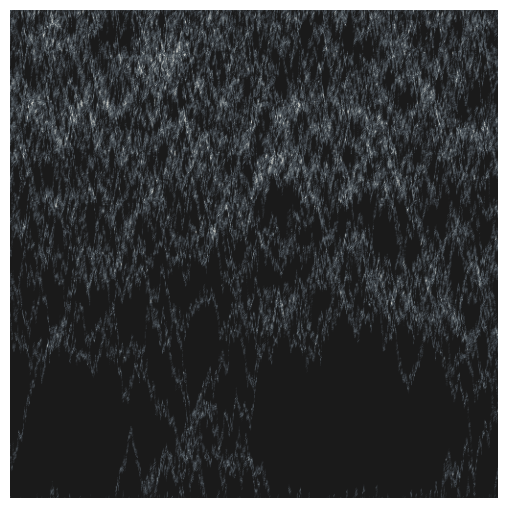
\includegraphics[width=0.32\linewidth]{../tex-src/images/flowImps3/flowl0r0.png} \\
   \begin{tabular}{c} \vspace{-12em} \\ \hspace{-1em}$\rho_M=0.50$\hspace{0em} \\  \\ \end{tabular} & 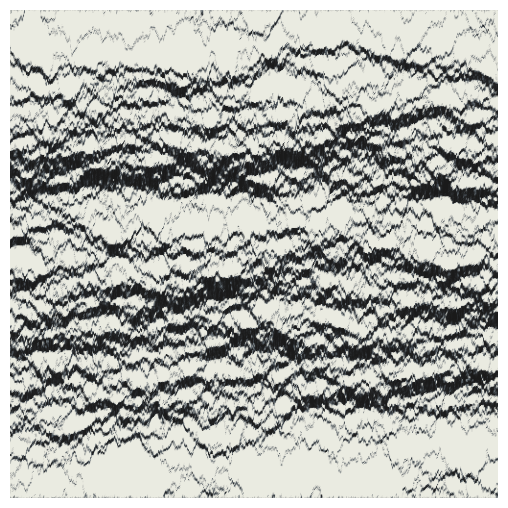
\includegraphics[width=0.32\linewidth]{../tex-src/images/flowImps2/flowl0r2.png} & 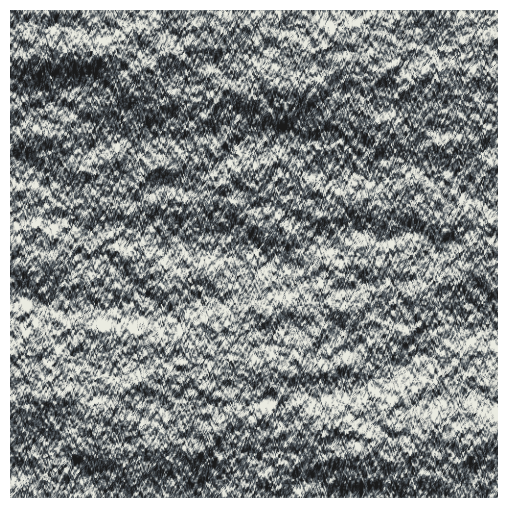
\includegraphics[width=0.32\linewidth]{../tex-src/images/flowImps2/flowl2r2.png}  & 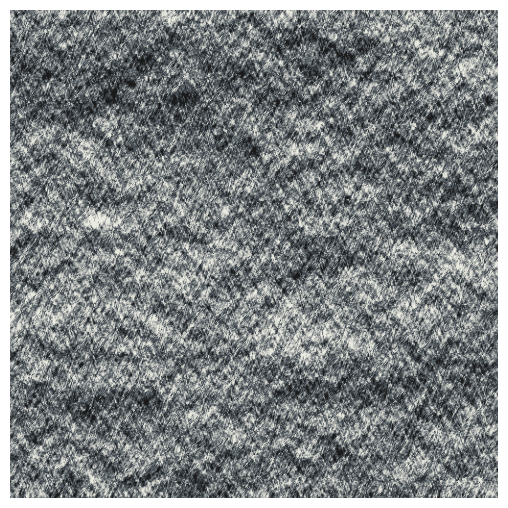
\includegraphics[width=0.32\linewidth]{../tex-src/images/flowImps3/flowl0r2.png} \\
   \begin{tabular}{c} \vspace{-12em} \\ \hspace{-1em}$\rho_M=0.95$\hspace{0em} \\  \\ \end{tabular} & 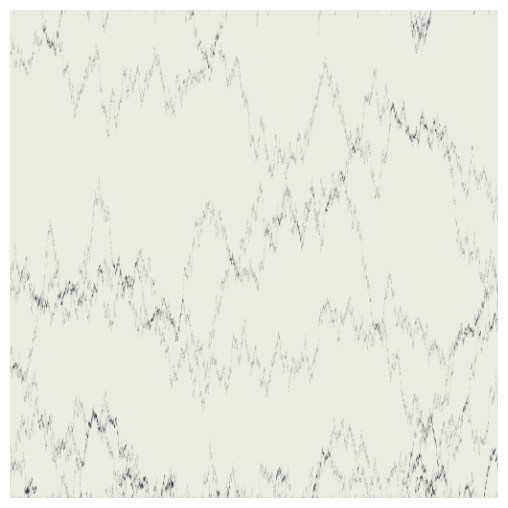
\includegraphics[width=0.32\linewidth]{../tex-src/images/flowImps2/flowl0r4.png} & 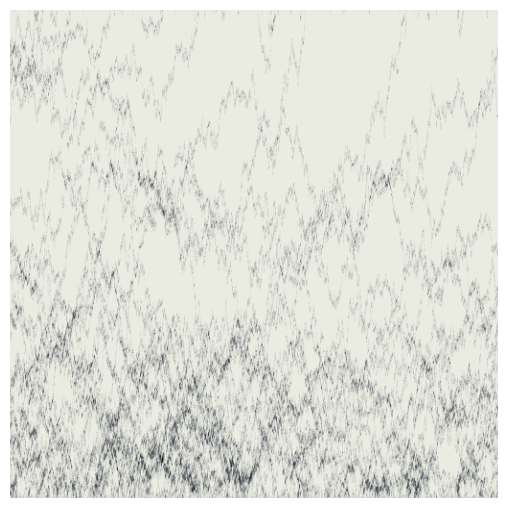
\includegraphics[width=0.32\linewidth]{../tex-src/images/flowImps2/flowl2r4.png}  & 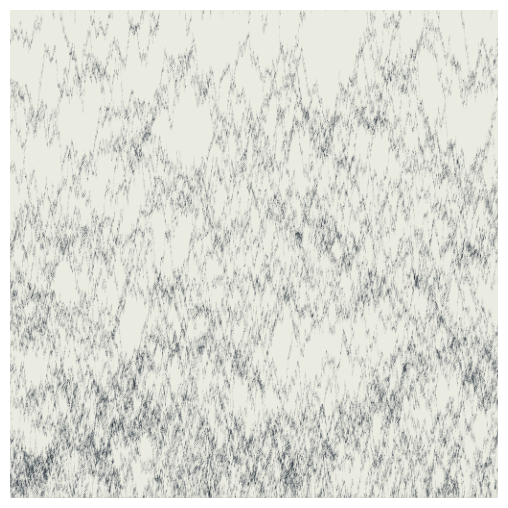
\includegraphics[width=0.32\linewidth]{../tex-src/images/flowImps3/flowl0r4.png} \\
   \end{tabular}
\hspace{-1em}
&
\end{tabular}
\end{figure*}
A few observations:

When $\lambda$ is extremely low (left), the medium consists of solid blocks surrounded by empty spaces containing a dilute
gas of particles; as we alter the overall density, all that changes is the thicknesses of these blocks.   Thus the breakdown of MFT
is revealed as a decomposition into two regions, of low and high density, each of which allows similar flow rate.  The MFT solution, which assumed
intermediate density and gave negative diffusion constant, is revealed to be unstable.
The case $\lambda = 1$ (right) is just excluded Brownian motion, and is included here for comparison.
The most interesting images (centre) are those for the intermediate $(\rho_M , \lambda)$; here we see a ``lumpy'' or ``foamy'' structure, in which small blocks
of particles are being constantly created and destroyed whilst a rather minimal flow occurs across the system.
The simulation did not show any hard phase transition as we vary $\rho_M, \lambda)$; rather, it seems that this ``foamy''
behaviour is part of a continuous range between the extremes, containing medium-range correlations between particles.
Unfortunately, computing equal-time correlation functions to the accuracy required
to draw conclusions about these correlations has proven to be extremely difficult, so we cannot find a quantitative description of the foam beyond the averages properties in Figures~\ref{fig:lambdaScans, fig:constDens, fig:diffCoeff}.
In all images in Figure~\ref{fig:flowPatterns}, long straight segments of white of black can be seen.  The represent coherent motion at a characteristic velocity given by their gradient. There is nothing in the MFT to suggest what this velocity
should be, and it is much smaller than the simulated system's length divided by the elapsed time,  $\frac{L}{T}$, thus it must be an emergent property arising from correlated motion of self-assembled regions of  high- or low-density material.

When $\lambda$ is extremely low, the medium consists of solid blocks surrounded by empty spaces containing a dilute gas of particles; as we alter the overall density,
all that changes is the thicknesses of these blocks. The case $\lambda=1$ is just excluded Brownian motion, and is included here for comparison. The most interesting images are those for the intermediate $(\rho_M , \lambda)$; here
we see a ``lumpy'' or ``foamy'' structure, in which small blocks of particles are being constantly created and destroyed whilst a rather minimal flow occurs across the system.
We do not think that there is any hard phase transition as we vary $(\rho_M , \lambda)$; rather, it seems that this ``foamy'' behaviour is part of a continuous range of phenomena between the extremes, containing medium-range correlations between
particles. However, numerically computing equal-time correlation functions to the accuracy required to draw conclusions about these correlations has proven to be extremely difficult, so we cannot speak in quantitative terms about them.
\iffalse
\subsection{Correlation Functions}
Whilst we're calculating flow rates, we can also use our \texttt{KMCLib} code to calculate the equal time 2-point correlation function
$C(x) = \left\langle \rho(x)\rho(0) \right\rangle - \left\langle \rho(x) \right\rangle \left\langle \rho(0) \right\rangle $.
We can calculate the same quantity in a finite periodic ring analytically, and in both the analytic and numerical cases we may attempt to extract a correlation length by (curve-fitting / Laplace transform);
hence we can check whether having a steady flow through the system causes any structural effects.}
\fi